\documentclass[main.tex]{subfiles}
\begin{document}


\begin{frame}{Content}

\begin{itemize}
    \item Question: Do elephants slow down to give birth and nurture their newborns?
    \item What are hidden Markov models (HMMs)?
    \item How to fit HMMs to data.
    \item Answer: Do elephants slow down to give birth and nurture their newborns? 
\end{itemize}
    
\end{frame}

\begin{frame}
\frametitle{Hypothesis: animals have a series of imperfectly observed / unobserved states which represent \textit{distinct} behaviours}

\begin{figure}
    \centering
    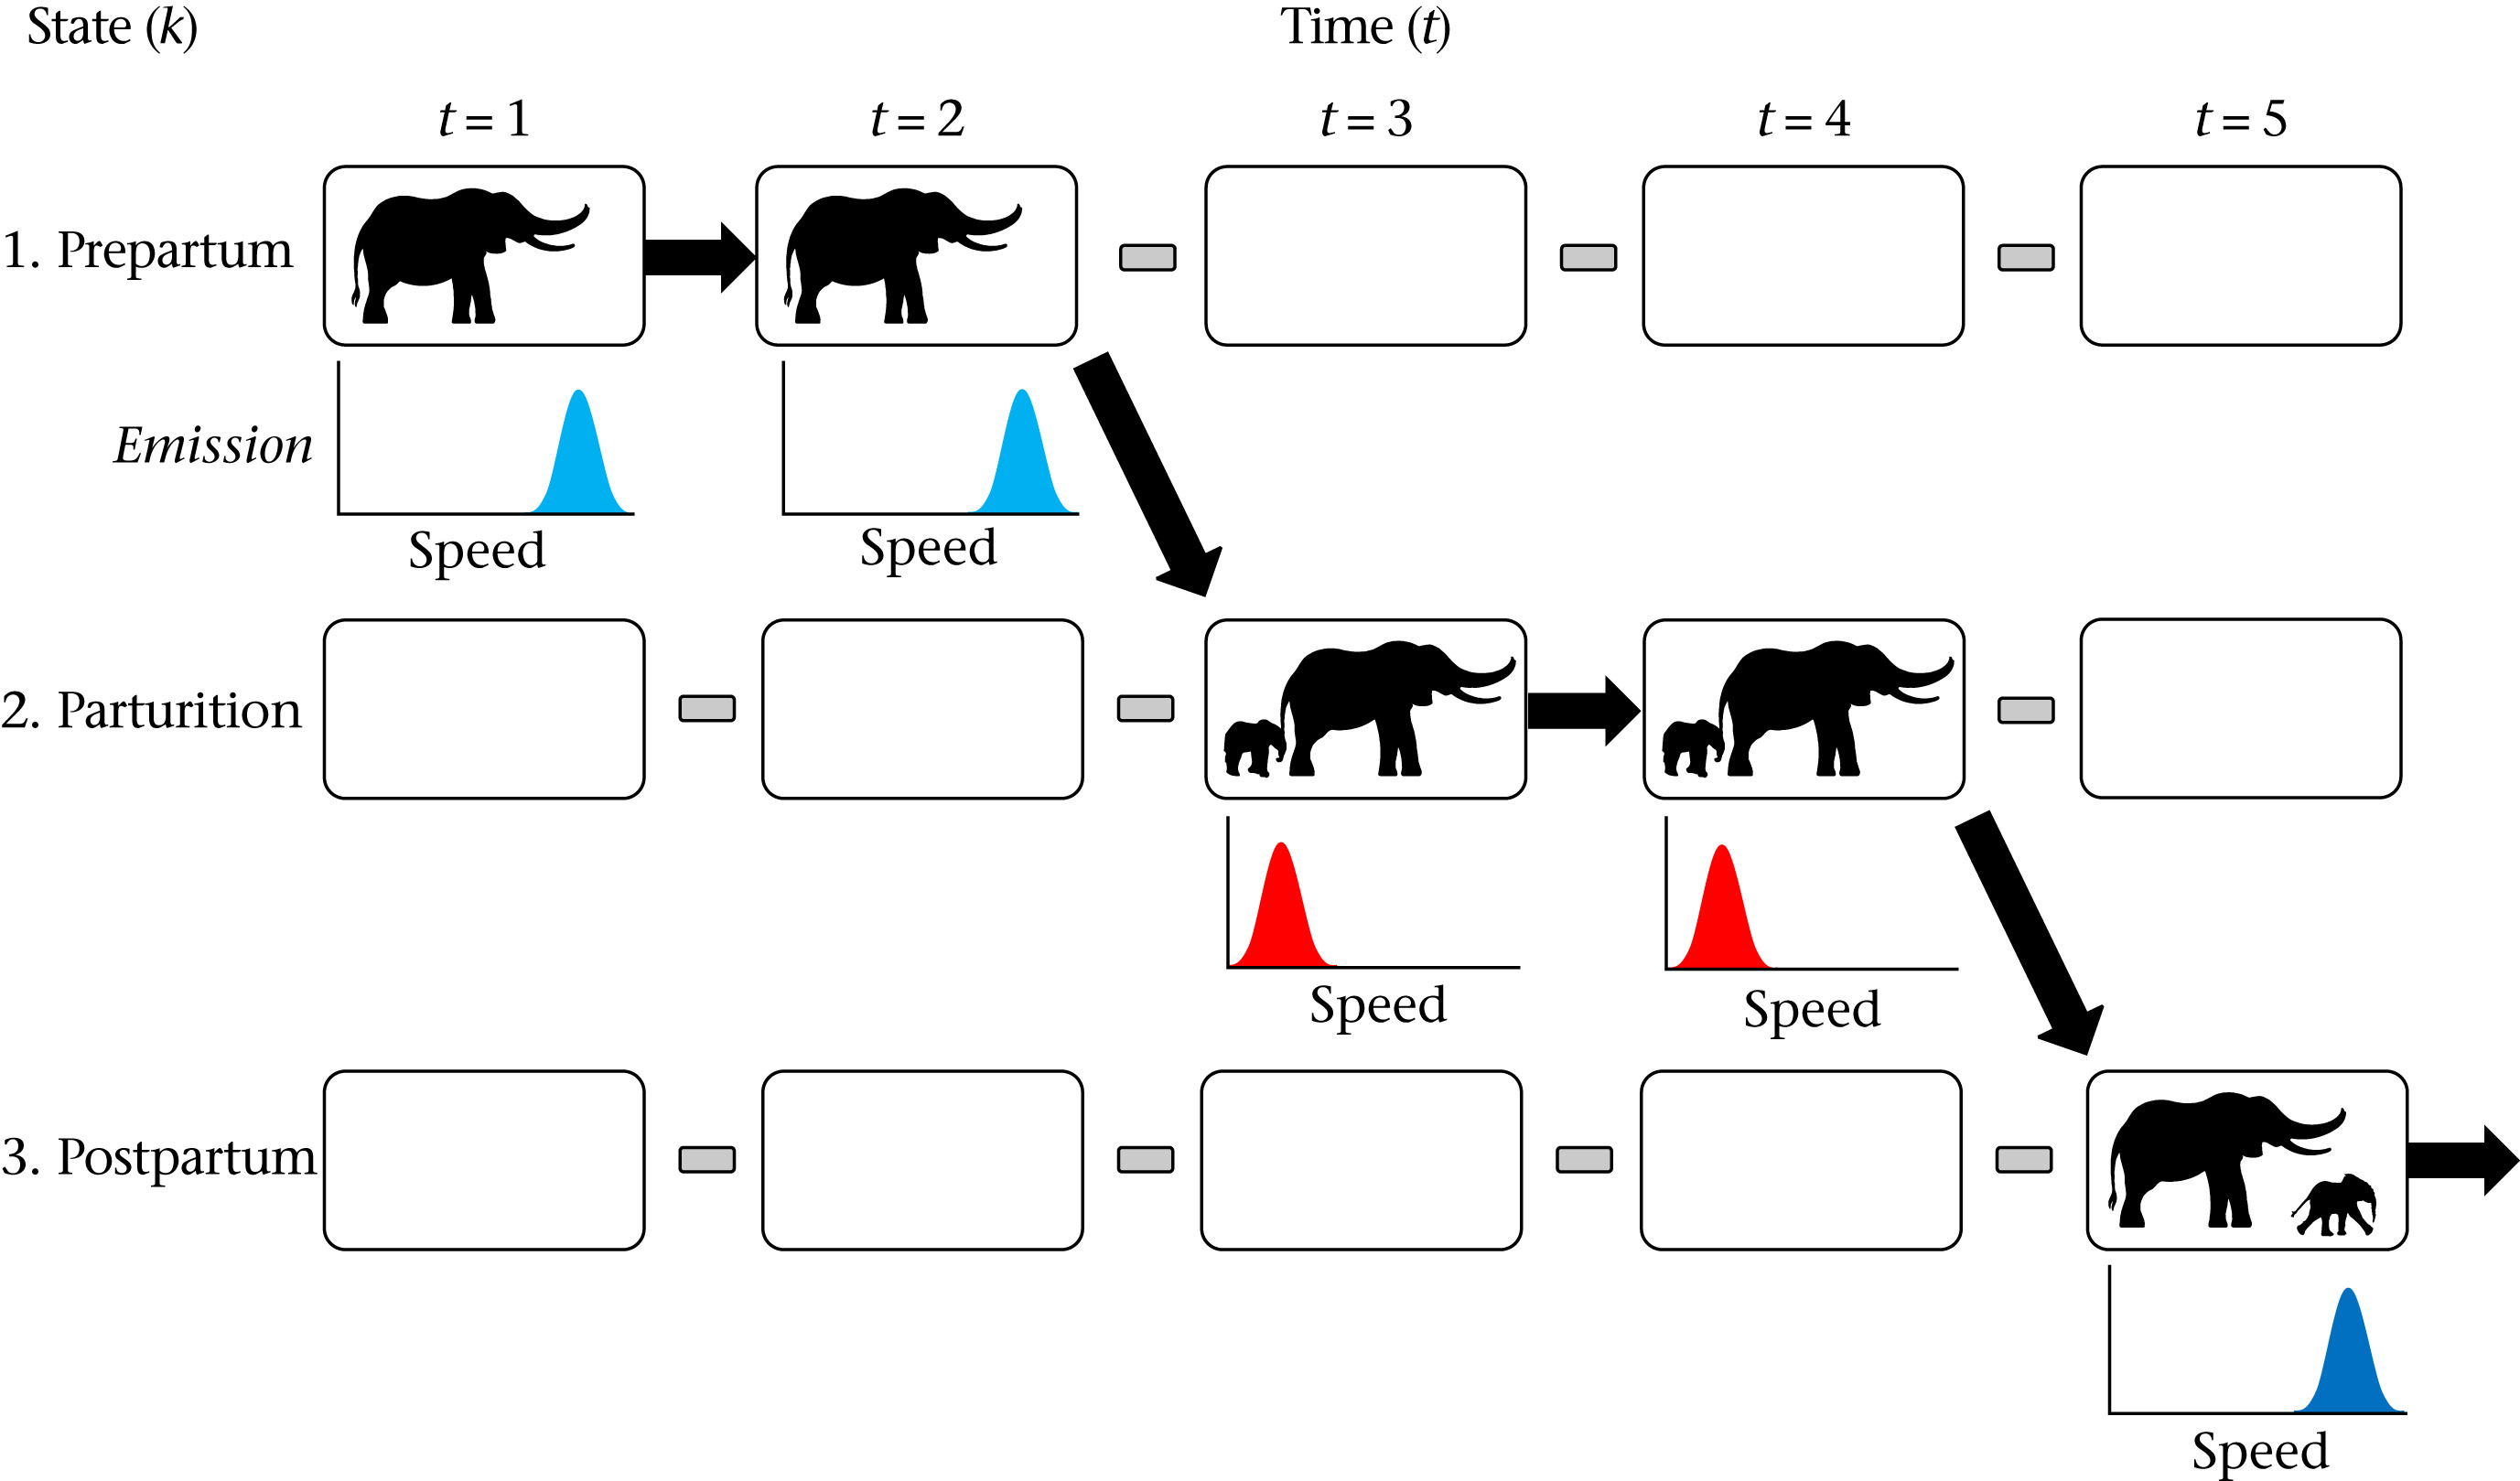
\includegraphics[width=0.8\textwidth]{figures/elephant_parturition.jpg}
    \caption{From Taylor et al. 2022, ``Movement behaviour after birth demonstrates precocial abilities of African savannah elephant, Loxodonta africana, calves''.}
    \label{fig:enter-label}
\end{figure}

\end{frame}

\begin{frame}
\frametitle{Aim of analysis: use data to uncover states and behaviours from imperfect data}

Goals:

\begin{itemize}
    \item Determine an animal state at each point in time
    \item Find an association between states and observations
\end{itemize}
    
\end{frame}

\begin{frame}
\frametitle{Example: GPS collared elephants (here, Luna)}

\begin{figure}
    \centering
    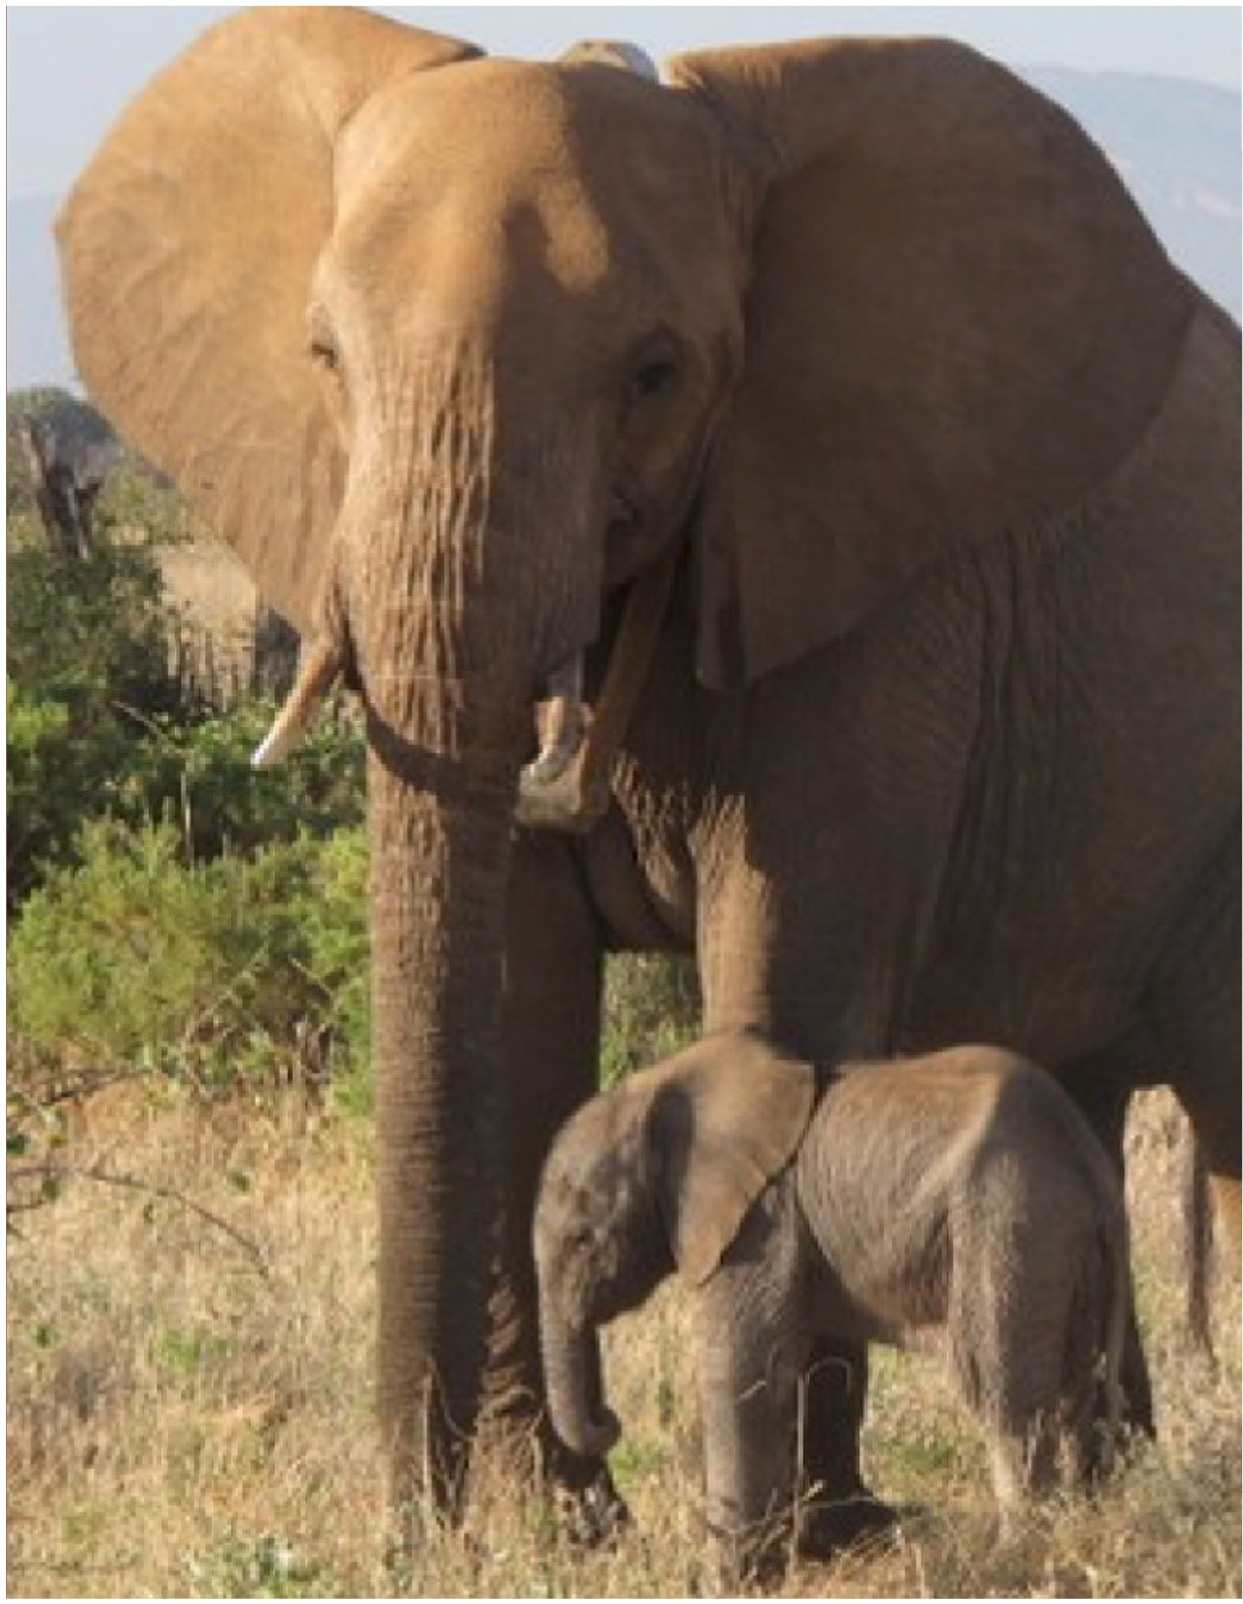
\includegraphics[width=0.5\textwidth]{figures/luna.jpg}
    \caption{From Taylor et al. 2022, ``Movement behaviour after birth demonstrates precocial abilities of African savannah elephant, Loxodonta africana, calves''.}
\end{figure}
    
\end{frame}

\begin{frame}
\frametitle{Use GPS fixes to determine speed}

\begin{figure}
    \centering
    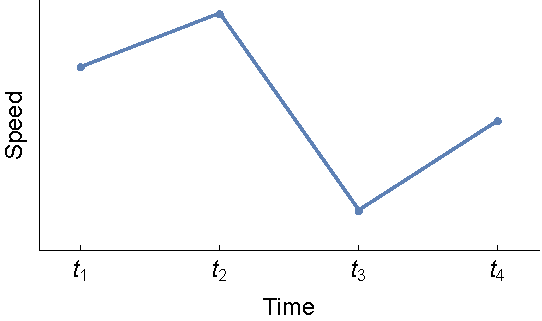
\includegraphics[width=0.8\textwidth]{figures/hmm_time_series.pdf}
\end{figure}
    
\end{frame}

\begin{frame}
\frametitle{An introduction to hidden Markov models (HMMs)}

Let's suppose for simplicity, that an animal can be in one of two behavioural states:

\vspace{0.5cm}

\begin{itemize}
    \item \textit{Migrating} ($m$): animals move directedly at a fast pace
    \item \textit{Foraging} ($f$): animals move slowly as they explore an area
\end{itemize}

\vspace{0.5cm}

Replace with two pictures
    
\end{frame}

\begin{frame}
\frametitle{Emission distributions}
Suppose the animals are collared with GPS machines, allowing us to measure the average animal speed in discrete intervals, $\text{Speed}(xt)$, where $x\in\{m,f\}$.

\vspace{0.5cm}

\begin{itemize}
    \item \textit{Migrating} ($m$): $\text{Speed}(t)\sim \text{normal}(\mu_m,\sigma_m)$
    \item \textit{Foraging} ($f$): $\text{Speed}(t)\sim \text{normal}(\mu_f,\sigma_f)$
\end{itemize}

\begin{figure}
    \centering
    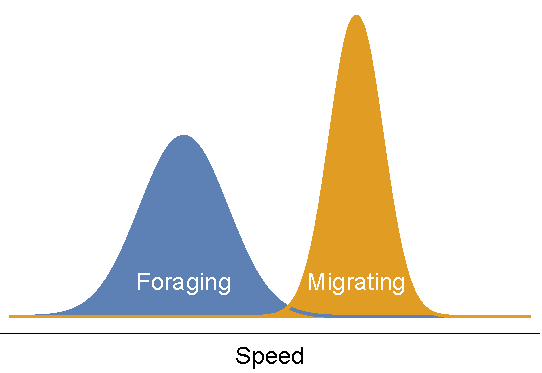
\includegraphics[width=0.55\textwidth]{figures/foraging_migrating.pdf}
\end{figure}
    
\end{frame}

\begin{frame}
\frametitle{A model for how observations are generated}

\begin{center}
\begin{tikzpicture}[node distance=2cm, block/.style={draw, minimum width=1cm, minimum height=1cm}]

  % First row
  \node[block] (A1) {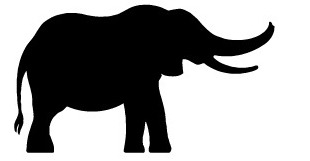
\includegraphics[width=1cm]{figures/elephant.jpg}};
  \node[block, right of=A1] (A2) {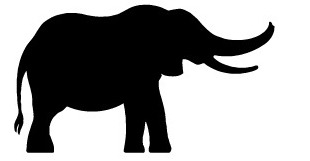
\includegraphics[width=1cm]{figures/elephant.jpg}};
  \node[block, right of=A2] (A3) {};
  \node[block, right of=A3] (A4) {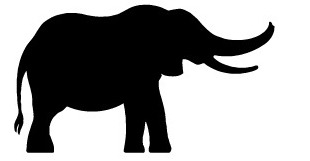
\includegraphics[width=1cm]{figures/elephant.jpg}};

  % Second row
  \node[block, below of=A1] (B1) {};
  \node[block, right of=B1] (B2) {};
  \node[block, right of=B2] (B3) {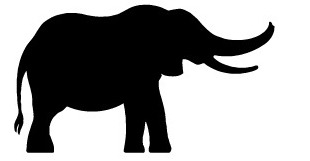
\includegraphics[width=1cm]{figures/elephant.jpg}};
  \node[block, right of=B3] (B4) {};

  % ghost nodes
  \node[coordinate, left of=A1] (J1) {};
  \node[] at (J1) {Migrating:};
  \node[coordinate, left of=B1] (J2) {};
  \node[] at (J2) {Foraging:};
  \node[coordinate, above of=A1, yshift=-0.5cm] (G1) {};
  \node[above] at (G1) {Speed($t_1$)};
  \node[coordinate, above of=A2, yshift=-0.5cm] (G2) {};
  \node[above] at (G2) {Speed($t_2$)};
  \node[coordinate, above of=A3, yshift=-0.5cm] (G3) {};
  \node[coordinate, above of=A4, yshift=-0.5cm] (G4) {};
  \node[above] at (G4) {Speed($t_4$)};
  \node[coordinate, below of=B1, yshift=0.5cm] (H1) {};
  \node[coordinate, below of=B2, yshift=0.5cm] (H2) {};
  \node[coordinate, below of=B3, yshift=0.5cm] (H3) {};
  \node[below] at (H3) {Speed($t_3$)};
  \node[coordinate, below right of=B4] (H4) {};

  % Horizontal arrows
  \draw[->, line width=2pt] (A1.east) -- (A2.west);

  % diagonal to blocks
  \draw[->, line width=2pt] (A2.south east) -- (B3.north);
  \draw[->, line width=2pt] (B3.north east) -- (A4.south);

  % Diagonal arrows
  \draw[->, line width=2pt, orange] (A1.north) -- (G1.west);
  \draw[->, line width=2pt, orange] (A2.north) -- (G2.west);
  \draw[->, line width=2pt, orange] (A4.north) -- (G4.west);
  \draw[->, line width=2pt, blue] (B3.south) -- (H3.west);


  \node[above of=G1,  yshift=-1cm] (timeStart) {};
  \node[above of=G4,  yshift=-1cm] (timeEnd) {};
  \draw[->] (timeStart.west) -- node[above] {Time} (timeEnd.east);

\end{tikzpicture}
\end{center}

\end{frame}

\begin{frame}
\frametitle{The data we actually observe}

\begin{figure}
    \centering
    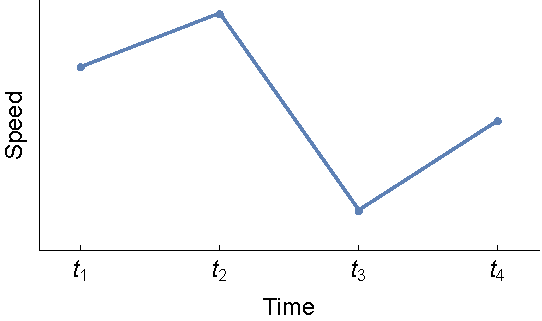
\includegraphics[width=0.8\textwidth]{figures/hmm_time_series.pdf}
\end{figure}
    
\end{frame}

\begin{frame}
\frametitle{The large space of possibilities}

\begin{center}
\begin{tikzpicture}[node distance=2cm, block/.style={draw, minimum width=1cm, minimum height=1cm}]

  % First row
  \node[block] (A1) {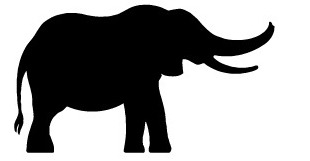
\includegraphics[width=1cm]{figures/elephant.jpg}};
  \node[block, right of=A1] (A2) {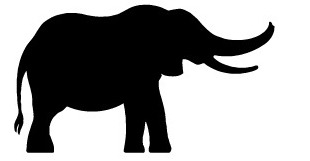
\includegraphics[width=1cm]{figures/elephant.jpg}};
  \node[block, right of=A2] (A3) {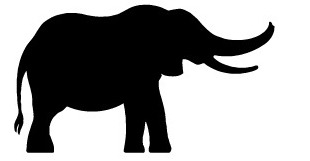
\includegraphics[width=1cm]{figures/elephant.jpg}};
  \node[block, right of=A3] (A4) {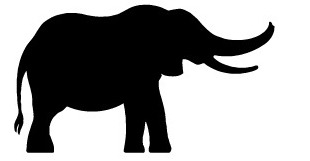
\includegraphics[width=1cm]{figures/elephant.jpg}};

  % Second row
  \node[block, below of=A1] (B1) {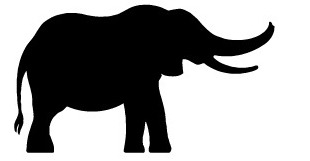
\includegraphics[width=1cm]{figures/elephant.jpg}};
  \node[block, right of=B1] (B2) {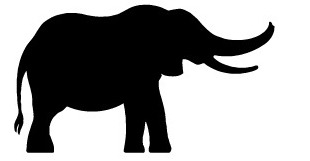
\includegraphics[width=1cm]{figures/elephant.jpg}};
  \node[block, right of=B2] (B3) {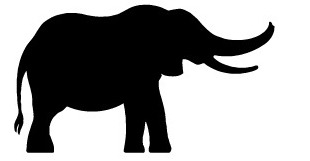
\includegraphics[width=1cm]{figures/elephant.jpg}};
  \node[block, right of=B3] (B4) {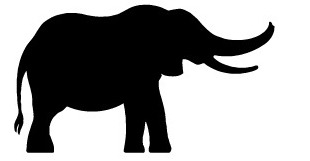
\includegraphics[width=1cm]{figures/elephant.jpg}};

  % ghost nodes
  \node[coordinate, left of=A1] (J1) {};
  \node[] at (J1) {Migrating:};
  \node[coordinate, left of=B1] (J2) {};
  \node[] at (J2) {Foraging:};
  \node[coordinate, above of=A1, yshift=-0.5cm] (G1) {};
  \node[above] at (G1) {Speed($t_1$)};
  \node[coordinate, above of=A2, yshift=-0.5cm] (G2) {};
  \node[above] at (G2) {Speed($t_2$)};
  \node[coordinate, above of=A3, yshift=-0.5cm] (G3) {};
  \node[above] at (G3) {Speed($t_3$)};
  \node[coordinate, above of=A4, yshift=-0.5cm] (G4) {};
  \node[above] at (G4) {Speed($t_4$)};
  \node[coordinate, below of=B1, yshift=0.5cm] (H1) {};
  \node[below] at (H1) {Speed($t_1$)};
  \node[coordinate, below of=B2, yshift=0.5cm] (H2) {};
  \node[below] at (H2) {Speed($t_2$)};
  \node[coordinate, below of=B3, yshift=0.5cm] (H3) {};
  \node[below] at (H3) {Speed($t_3$)};
  \node[coordinate, below of=B4, yshift=0.5cm] (H4) {};
  \node[below] at (H4) {Speed($t_4$)};

  % Horizontal arrows
  \draw[->, line width=2pt] (A1.east) -- (A2.west);
  \draw[->, line width=2pt] (A2.east) -- (A3.west);
  \draw[->, line width=2pt] (A3.east) -- (A4.west);
  \draw[->, line width=2pt] (B1.east) -- (B2.west);
  \draw[->, line width=2pt] (B2.east) -- (B3.west);
  \draw[->, line width=2pt] (B3.east) -- (B4.west);

  % diagonal to blocks
  \draw[->, line width=2pt] (A1.south east) -- (B2.north);
  \draw[->, line width=2pt] (A2.south east) -- (B3.north);
  \draw[->, line width=2pt] (A3.south east) -- (B4.north);
  \draw[->, line width=2pt] (B1.north east) -- (A2.south);
  \draw[->, line width=2pt] (B2.north east) -- (A3.south);
  \draw[->, line width=2pt] (B3.north east) -- (A4.south);

  % vertical arrows
  \draw[->, line width=2pt, orange] (A1.north) -- (G1.west);
  \draw[->, line width=2pt, orange] (A2.north) -- (G2.west);
  \draw[->, line width=2pt, orange] (A3.north) -- (G3.west);
  \draw[->, line width=2pt, orange] (A4.north) -- (G4.west);
  \draw[->, line width=2pt, blue] (B1.south) -- (H1.west);
  \draw[->, line width=2pt, blue] (B2.south) -- (H2.west);
  \draw[->, line width=2pt, blue] (B3.south) -- (H3.west);
  \draw[->, line width=2pt, blue] (B4.south) -- (H4.west);


  \node[above of=G1, yshift=-1cm] (timeStart) {};
  \node[above of=G4, yshift=-1cm] (timeEnd) {};
  \draw[->] (timeStart.west) -- node[above] {Time} (timeEnd.east);

\end{tikzpicture}
\end{center}
    
\end{frame}

\begin{frame}
\frametitle{Start with data}

\begin{center}
\begin{tikzpicture}[node distance=2cm, block/.style={draw, minimum width=1cm, minimum height=1cm}]

  % First row
  \node[block, white] (A1) {};
  \node[block, right of=A1, white] (A2) {};
  \node[block, right of=A2, white] (A3) {};
  \node[block, right of=A3, white] (A4) {};

  % Second row
  \node[block, below of=A1, white] (B1) {};
  \node[block, right of=B1, white] (B2) {};
  \node[block, right of=B2, white] (B3) {};
  \node[block, right of=B3, white] (B4) {};

  % ghost nodes
  \node[coordinate, left of=A1] (J1) {};
  \node[coordinate, left of=B1] (J2) {};
  \node[coordinate, above of=A1, yshift=-0.5cm] (G1) {};
  \node[above] at (G1) {Speed($t_1$)};
  \node[coordinate, above of=A2, yshift=-0.5cm] (G2) {};
  \node[above] at (G2) {Speed($t_2$)};
  \node[coordinate, above of=A3, yshift=-0.5cm] (G3) {};
  \node[above] at (G3) {Speed($t_3$)};
  \node[coordinate, above of=A4, yshift=-0.5cm] (G4) {};
  \node[above] at (G4) {Speed($t_4$)};
  \node[coordinate, below of=B1, yshift=0.5cm] (H1) {};
  \node[coordinate, below of=B2, yshift=0.5cm] (H2) {};
  \node[coordinate, below of=B3, yshift=0.5cm] (H3) {};
  \node[coordinate, below of=B4, yshift=0.5cm] (H4) {};
  \node[below] at (H1) {Speed($t_1$)};
  \node[below] at (H2) {Speed($t_2$)};
  \node[below] at (H3) {Speed($t_3$)};
  \node[below] at (H4) {Speed($t_4$)};


  \node[above of=G1, yshift=-1cm] (timeStart) {};
  \node[above of=G4, yshift=-1cm] (timeEnd) {};
  \draw[->] (timeStart.west) -- node[above] {Time} (timeEnd.east);

\end{tikzpicture}
\end{center}
    
\end{frame}

\begin{frame}
\frametitle{Use data to estimate states and transitions}

\begin{center}
\begin{tikzpicture}[node distance=2cm, block/.style={draw, minimum width=1cm, minimum height=1cm}]

  % First row
  \node[block] (A1) {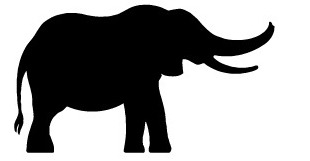
\includegraphics[width=1cm]{figures/elephant.jpg}};
  \node[block, right of=A1] (A2) {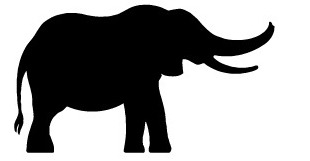
\includegraphics[width=1cm]{figures/elephant.jpg}};
  \node[block, right of=A2] (A3) {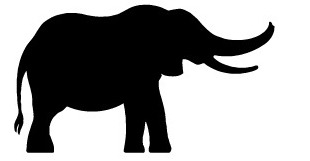
\includegraphics[width=1cm]{figures/elephant.jpg}};
  \node[block, right of=A3] (A4) {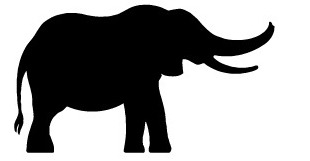
\includegraphics[width=1cm]{figures/elephant.jpg}};

  % Second row
  \node[block, below of=A1] (B1) {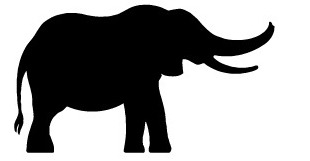
\includegraphics[width=1cm]{figures/elephant.jpg}};
  \node[block, right of=B1] (B2) {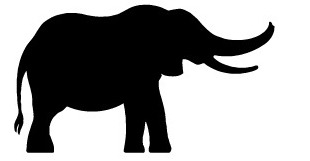
\includegraphics[width=1cm]{figures/elephant.jpg}};
  \node[block, right of=B2] (B3) {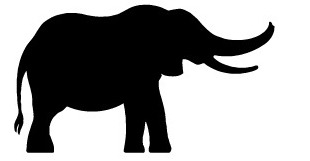
\includegraphics[width=1cm]{figures/elephant.jpg}};
  \node[block, right of=B3] (B4) {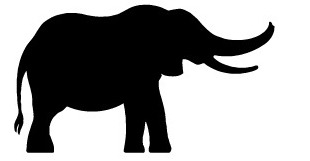
\includegraphics[width=1cm]{figures/elephant.jpg}};
  

  % ghost nodes
  \node[coordinate, left of=A1] (J1) {};
  \node[] at (J1) {Migrating:};
  \node[coordinate, left of=B1] (J2) {};
  \node[] at (J2) {Foraging:};
  \node[coordinate, above of=A1, yshift=-0.5cm] (G1) {};
  \node[above] at (G1) {Speed($t_1$)};
  \node[coordinate, above of=A2, yshift=-0.5cm] (G2) {};
  \node[above] at (G2) {Speed($t_2$)};
  \node[coordinate, above of=A3, yshift=-0.5cm] (G3) {};
  \node[above] at (G3) {Speed($t_3$)};
  \node[coordinate, above of=A4, yshift=-0.5cm] (G4) {};
  \node[above] at (G4) {Speed($t_4$)};
  \node[coordinate, below of=B1, yshift=0.5cm] (H1) {};
  \node[below] at (H1) {Speed($t_1$)};
  \node[coordinate, below of=B2, yshift=0.5cm] (H2) {};
  \node[below] at (H2) {Speed($t_2$)};
  \node[coordinate, below of=B3, yshift=0.5cm] (H3) {};
  \node[below] at (H3) {Speed($t_3$)};
  \node[coordinate, below of=B4, yshift=0.5cm] (H4) {};
  \node[below] at (H4) {Speed($t_4$)};

  % Horizontal arrows
  \draw[->, line width=2pt, opacity=0.5] (A1.east) -- (A2.west);
  \draw[->, line width=2pt, opacity=0.1] (A2.east) -- (A3.west);
  \draw[->, line width=2pt, opacity=0.1] (A3.east) -- (A4.west);
  \draw[->, line width=2pt, opacity=0.1] (B1.east) -- (B2.west);
  \draw[->, line width=2pt, opacity=0.1] (B2.east) -- (B3.west);
  \draw[->, line width=2pt, opacity=0.1] (B3.east) -- (B4.west);

  % diagonal to blocks
  \draw[->, line width=2pt, opacity=0.1] (A1.south east) -- (B2.north);
  \draw[->, line width=2pt, opacity=0.5] (A2.south east) -- (B3.north);
  \draw[->, line width=2pt, opacity=0.1] (A3.south east) -- (B4.north);
  \draw[->, line width=2pt, opacity=0.1] (B1.north east) -- (A2.south);
  \draw[->, line width=2pt, opacity=0.1] (B2.north east) -- (A3.south);
  \draw[->, line width=2pt] (B3.north east) -- (A4.south);

  % vertical arrows
  \draw[<-, line width=2pt, orange] (A1.north) -- (G1.west);
  \draw[<-, line width=2pt, orange] (A2.north) -- (G2.west);
  \draw[<-, line width=2pt, orange] (A3.north) -- (G3.west);
  \draw[<-, line width=2pt, orange] (A4.north) -- (G4.west);
  \draw[<-, line width=2pt, blue] (B1.south) -- (H1.west);
  \draw[<-, line width=2pt, blue] (B2.south) -- (H2.west);
  \draw[<-, line width=2pt, blue] (B3.south) -- (H3.west);
  \draw[<-, line width=2pt, blue] (B4.south) -- (H4.west);


  \node[above of=G1, yshift=-1cm] (timeStart) {};
  \node[above of=G4, yshift=-1cm] (timeEnd) {};
  \draw[->] (timeStart.west) -- node[above] {Time} (timeEnd.east);

\end{tikzpicture}
\end{center}
    
\end{frame}


\begin{frame}
\frametitle{Mathematical description: emission distributions}

\begin{equation}
    \text{Speed}(t, x_t) \overset{\text{iid}}{\sim} \text{normal}(\mu_{x_t}, \sigma_{x_t}),
\end{equation}

where $x[t]\in\{m,f\}$.

\vspace{0.5cm}

This is just a (Gaussian) clustering model.
    
\end{frame}

\begin{frame}
\frametitle{Mathematical description: state transitions}

In HMMs, we typically assume that the state transitions are (1st order) Markovian:
%
\begin{equation}
    p(X_t = a| X_{t-1}, X_{t-2},...,X_0) = p(X_t = a| X_{t-1}),
\end{equation}
%
which means that state transitions can be represented by a $2\times 2$ matrix:
%
\begin{equation}
        \begin{bmatrix} p_{m,m} & p_{m,f}\\ p_{f,m} & p_{f,f} \end{bmatrix} := \begin{bmatrix} p(X_t=m | X_{t-1}=m) & p(X_t=f | X_{t-1}=m) \\ p(X_t=m | X_{t-1}=f) & p(X_t=f | X_{t-1}=f) \end{bmatrix}.
\end{equation}
%
    
\end{frame}

\begin{frame}
\frametitle{Inference problem}

We do not know:

\begin{itemize}
    \item The emission distribution parameters, $\theta := (\mu_f,\mu_m,\sigma_f,\sigma_m),$ 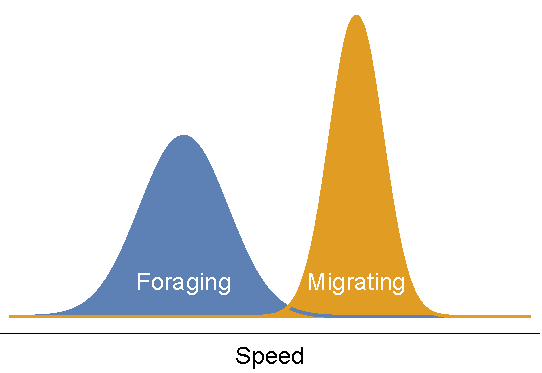
\includegraphics[width=2.5cm]{figures/foraging_migrating.pdf}
    \item The states, \begin{center}
\begin{tikzpicture}[node distance=1cm, block/.style={draw, minimum width=0.5cm, minimum height=0.5cm}]

  % First row
  \node[block] (A1) {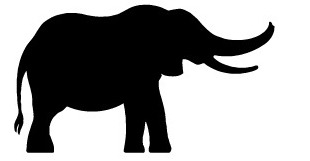
\includegraphics[width=0.5cm]{figures/elephant.jpg}};
  \node[block, right of=A1] (A2) {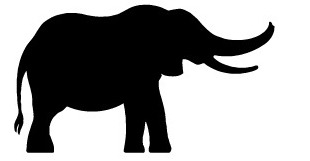
\includegraphics[width=0.5cm]{figures/elephant.jpg}};
  \node[block, right of=A2] (A3) {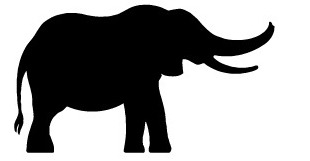
\includegraphics[width=0.5cm]{figures/elephant.jpg}};
  \node[block, right of=A3] (A4) {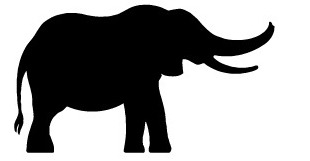
\includegraphics[width=0.5cm]{figures/elephant.jpg}};

  % Second row
  \node[block, below of=A1] (B1) {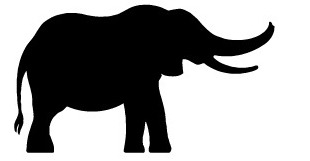
\includegraphics[width=0.5cm]{figures/elephant.jpg}};
  \node[block, right of=B1] (B2) {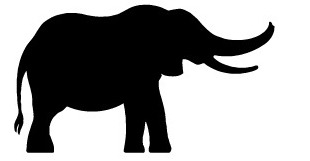
\includegraphics[width=0.5cm]{figures/elephant.jpg}};
  \node[block, right of=B2] (B3) {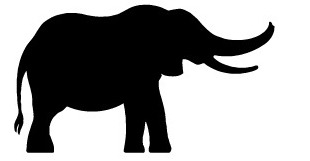
\includegraphics[width=0.5cm]{figures/elephant.jpg}};
  \node[block, right of=B3] (B4) {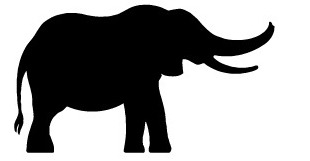
\includegraphics[width=0.5cm]{figures/elephant.jpg}};

  % Horizontal arrows
  \draw[->, line width=1pt, opacity=1] (A1.east) -- (A2.west);
  \draw[->, line width=1pt, opacity=1] (A2.east) -- (A3.west);
  \draw[->, line width=1pt, opacity=1] (A3.east) -- (A4.west);
  \draw[->, line width=1pt, opacity=1] (B1.east) -- (B2.west);
  \draw[->, line width=1pt, opacity=1] (B2.east) -- (B3.west);
  \draw[->, line width=1pt, opacity=1] (B3.east) -- (B4.west);

  % diagonal to blocks
  \draw[->, line width=1pt, opacity=1] (A1.south east) -- (B2.north);
  \draw[->, line width=1pt, opacity=1] (A2.south east) -- (B3.north);
  \draw[->, line width=1pt, opacity=1] (A3.south east) -- (B4.north);
  \draw[->, line width=1pt, opacity=1] (B1.north east) -- (A2.south);
  \draw[->, line width=1pt, opacity=1] (B2.north east) -- (A3.south);
  \draw[->, line width=1pt] (B3.north east) -- (A4.south);

\end{tikzpicture}
\end{center}
\item The transition probability matrix, \begin{equation}
    \begin{bmatrix} p_{m,m} & p_{m,f}\\ p_{f,m} & p_{f,f} \end{bmatrix},
\end{equation}
\end{itemize}

and we want to estimate these from data.
    
\end{frame}

\end{document}

